\documentclass[12pt,letterpaper]{article}
\usepackage[utf8]{inputenc}
\usepackage{float, xcolor}

%----- Configuración del estilo del documento------%
\usepackage{graphicx, fancyhdr, lastpage}
\usepackage{enumitem, pifont}
\usepackage[left=2cm,right=2cm,top=1.8cm,bottom=2.3cm]{geometry}

\pagestyle{fancy}
\fancyhf{}
\rfoot{\textit{Página \thepage \hspace{1pt} de \pageref{LastPage}}}

%------ Paquetes matemáticos básicos --------%
\usepackage{amsmath, amssymb, amsthm}

\newcommand{\imp}{\rightarrow}
\newcommand{\vp}{\varphi}

\begin{document}

%------ Encabezado -------- %
\begin{center}
  \begin{minipage}{3cm}
    \begin{center}
      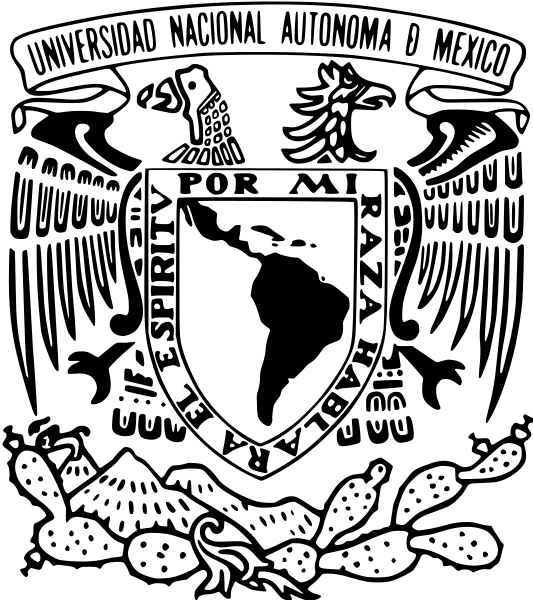
\includegraphics[height=3.4cm]{../unam_logo.png}
    \end{center}
  \end{minipage}\hfill
  \begin{minipage}{10cm}
    \begin{center}
      \textbf{\Large Universidad Nacional Autónoma de México}\\[0.2cm]
      \textbf{\large Facultad de Ciencias}\\[0.2cm]
      \textbf{Lógica Computacional | 2025-2}\\[0.4cm]
      \textbf{\Large Tarea 02}\\[0.1cm]
      \textbf{Docentes:}\\
      Noé Hernández \hspace{1em} Santiago Escamilla \hspace{1em} Ricardo López\\[0.3cm]
      \textbf{Autores:}\\
      Fernanda Ramírez Juárez \quad Ianluck Rojo Peña\\[0.3cm]
      \textbf{Fecha de entrega:} Martes 25 de febrero de 2025
    \end{center}
  \end{minipage}\hfill
  \begin{minipage}{3cm}
    \begin{center}
      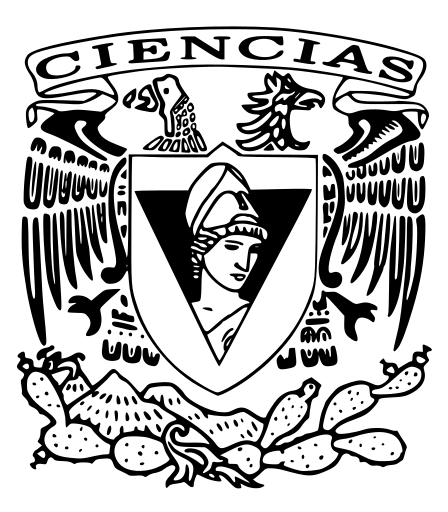
\includegraphics[height=3.4cm]{../fc_logo.png}
    \end{center}
  \end{minipage}
\end{center}

\bigskip
\hrule height 0.1pt
\bigskip

%------ Notas sobre la resolución --------%
\section*{Notas sobre la resolución.}

\begin{quote}
  \textbf{Nota general:}  
  Los ejercicios fueron resueltos en base a las notas de clase LcNota5.pdf y LcNota6.pdf.\\
  Junto con los comentarios impartidos en las sesiones del curso de la semana del 17 de febrero  al 21 de febrero del 2025, además de los días 24 y 25 de febrero.
\end{quote}

\bigskip
\hrule height 0.1pt
\bigskip

%------ Contenido -------- %
\section*{Resolución de Ejercicios.}

\begin{enumerate}
  
  % ---- Ejercicio 1 ----
  \item (1.5 pts.) El sumador que aparece a continuación implementa el par de fórmulas:
    \begin{figure}[H]
      \centering
      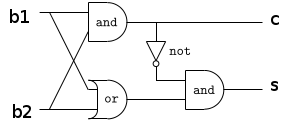
\includegraphics[width=0.5\textwidth]{circuit.png}
    \end{figure}

    \[
    s \leftrightarrow \neg (b_1 \land b_2) \land (b_1 \lor b_2), \quad c \leftrightarrow b_1 \land b_2
    \]
  
    Sea $C$ el conjunto que contiene al par de fórmulas anteriores.
    
    \begin{itemize}[label=\ding{112}]
    \item Muestre que $C \cup \{b_1 \land b_2 \land \neg s \land \neg c\}$ es insatisfacible usando resolución binaria.
    \item Exhiba una interpretación que satisfaga al conjunto $C \cup \{b_1 \land b_2 \land \neg s \land c\}$.
  \end{itemize}
    
  Explique el significado de estos dos puntos en términos del comportamiento del circuito.
  
  \bigskip
  % -- Respuesta --
  \subsubsection*{Forma Clausular y Resoluci\'{o}n Binaria.}
  Definimos el conjunto $C^*$ c\'{o}mo: $C^*$ = $C \cup \{b_1 \land b_2 \land \neg s \land \neg c\}$ \\
  Notemos que $\{b_1 \land b_2 \land \neg s \land \neg c\}$ ya est\'{a} en su Forma Clausular, por lo que tenemos que pasar las dos f\'{o}rmulas de $C$ a su Forma Clausular.
  
  \begin{itemize}[label=\textbullet]
  \item $s \leftrightarrow \neg (b_1 \land b_2) \land (b_1 \lor b_2)$:\\
    \\
    Eliminamos la doble implicaci\'{o}n $\leftrightarrow$
    \[
    \hspace{-0.9cm}
    s \leftrightarrow \neg (b_1 \land b_2) \land (b_1 \lor b_2)
    \equiv
    \Big(\neg s\lor \big(\neg (b_1 \land b_2) \land (b_1 \lor b_2) \big) \Big)
    \land
    \Big(s \lor \neg \big(\neg (b_1 \land b_2) \land (b_1 \lor b_2)\big) \Big)
    \]
    Distribuimos la negaci\'{o}n $\neg$, en las respectivas f\'{o}rmulas
    \[
    \equiv
    \Big(\neg s\lor \big((\neg b_1 \lor \neg b_2) \land (b_1 \lor b_2) \big) \Big)
    \land
    \Big(s \lor \big((b_1 \land b_2) \lor (\neg b_1 \land \neg b_2)\big) \Big)
    \]
    Distribuci\'{o}n de $\neg s$ para el lado izquierdo del $\land$ y distribuci\'{o}n de $(b_1 \land b_2)$ en $(\neg b_1 \land \neg b_2)$ del lado derecho
    \[
    \hspace{-0.5cm}
    \equiv
    \Big(\big(\neg s\lor (\neg b_1 \lor \neg b_2)\big) \land \big(\neg s \lor (b_1 \lor b_2) \big) \Big)
    \land
    \bigg(s \lor \Big(\big(b_1 \lor (\neg b_1 \land \neg b_2)\big)
    \land \big(b_2 \lor (\neg b_1 \land \neg b_2)\big)\Big)\bigg)
    \]
    N\'{o}tese que el lado derecho del $\land$ ya est\'{a} en su forma clausular, continuamos con la distribuci\'{o}n de $(\neg b_1 \land \neg b_2)$ en $b_1$ y $b_2$
    \[
    \hspace{-1.1cm}
    \equiv
    (\neg s\lor \neg b_1 \lor \neg b_2) \land (\neg s \lor b_1 \lor b_2)
    \land
    \bigg(s \lor \Big(\big((b_1 \lor \neg b_1) \land (b_1 \lor \neg b_2)\big)
    \land \big((b_2 \lor \neg b_1) \land (b_2 \lor \neg b_2)\big)\Big)\bigg)
    \]
    Eliminamos $(b_1 \lor \neg b_1)$ y $(b_2 \lor \neg b_2)$ pues son tautolog\'{i}as y no tiene sentido seguir ditribuyendo estas dos f\'{o}rmulas pues es hacer trabajo de m\'{a}s por darnos trivialidades, igualmente tomamos en cuenta la resoluci\'{o} del ejercico 4.\\
    Por lo que tenemos
    \[ 
    \hspace{0.5cm}
    \equiv
    (\neg s\lor \neg b_1 \lor \neg b_2) \land (\neg s \lor b_1 \lor b_2)
    \land
    \Big(s \lor \big((b_1 \lor \neg b_2)\land (b_2 \lor \neg b_1)\big)\Big)
    \]
    Distribuyendo s tenemos
    \[ 
    \hspace{0.5cm}
    \equiv
    (\neg s\lor \neg b_1 \lor \neg b_2) \land (\neg s \lor b_1 \lor b_2)
    \land
    \Big(\big(s \lor (b_1 \lor \neg b_2)\big) \land \big(s \lor (b_2 \lor \neg b_1)\big)\Big)
    \]
    \[
    \equiv
    (\neg s\lor \neg b_1 \lor \neg b_2) \land (\neg s \lor b_1 \lor b_2)
    \land
    (s \lor b_1 \lor \neg b_2) \land (s \lor b_2 \lor \neg b_1)
    \]
    Por lo que tenemos las premisas:
    \[
    1.\: \neg s, \neg b_{1}, \neg b_{2}
    \hspace{3mm} \big | \hspace{3mm}
    2.\: \neg s,\; b_{1},\; b_{2}
    \hspace{3mm} \big | \hspace{3mm}
    3.\: s,\; b_{1}, \neg b_{2}
    \hspace{3mm} \big | \hspace{3mm}
    4.\: s, \neg b_{1},\; b_{2}
    \]

  \item $c \leftrightarrow b_1 \land b_2$:\\
    \\
    Eliminamos la doble implicaci\'{o}n $\leftrightarrow$
    \[
    \hspace{-1cm}
    c \leftrightarrow b_1 \land b_2
    \equiv
    \big(\neg c \lor (b_1 \land b_2)\big) \land \big(c \lor \neg(b_1 \land b_2)\big)
    \]
    Del lado derecho distribuimos $\neg c$ y del lado izquierdo distribuimos la negaci\'{o}n
    \[
    \hspace{-1.5cm}
    \big(\neg c \lor (b_1 \land b_2)\big) \land \big(c \lor \neg(b_1 \land b_2)\big)
    \equiv
    (\neg c \lor b_1) \land (\neg c \lor b_2) \land (c \lor \neg b_1 \lor b_2)
    \]
    Por lo que tenemos las premisas:
    \[
    5.\: \neg c,\; b_1
    \hspace{3mm} \big | \hspace{3mm}
    6.\: \neg c,\; b_2
    \hspace{3mm} \big | \hspace{3mm}
    7.\: c, \neg b_{1}, \; b_2
    \]
    
  \end{itemize}

  Realizamos la Sustituci\'{o}n Binaria
  
  \begin{enumerate}[label=\arabic*.]
  \item $\neg s, \neg b_1, \neg b_2$ \hspace{0.4cm} Prem
  \item $\neg s, b_1, b_2$ \hspace{1cm} Prem
  \item $s, b_1, \neg b_2$ \hspace{1cm} Prem
  \item $s, \neg b_1, b_2$ \hspace{1cm} Prem
  \item $\neg c, b_1$ \hspace{1.5cm} Prem
  \item $\neg c, b_2$ \hspace{1.5cm} Prem
  \item $c, \neg b_1, \neg b_2$ \hspace{0.7cm} Prem
  \item $b_1$ \hspace{2.2cm} Prem
  \item $b_2$ \hspace{2.2cm} Prem
  \item $\neg s$ \hspace{2.1cm} Prem
  \item $\neg c$ \hspace{2.1cm} Prem
  \item $c, \neg b_2$ \hspace{1.6cm} Res(7, 8)
  \item $c$ \hspace{2.4cm} Res(12, 9)
  \item $\square$ \hspace{2.3cm} Res(13, 11)
  \end{enumerate}
  \[
  \therefore \;\; \text{El conjunto } C^* \text{ es insatisfacible pues hemos llegado a la cláusula vacía.}
  \]

  \subsubsection*{Interpretación satisfactible.}
  Definimos el conjunto $C^*$ c\'{o}mo: $C^*$ = $C \cup \{b_1 \land b_2 \land \neg s \land c\}$\\
  Es decir $C^* = \{s \leftrightarrow \neg (b_1 \land b_2) \land (b_1 \lor b_2), \quad c \leftrightarrow b_1 \land b_2, \quad b_1 \land b_2 \land \neg s \land c\}$\\
  Y as\'{i} tenemos la interpretaci\'{o}n:
  \[
  I(b_1) = I(b_2) = 1, \quad I(s) = 0 \rightarrow I(\neg s) = 1, \quad I(c) = 1
  \]
  La cual satisface al conjunto $C^*$:
  \[
  \hspace{-2cm}
  I(s \leftrightarrow \neg (b_1 \land b_2) \land (b_1 \lor b_2)) = I(s) = I(\neg (b_1 \land b_2) \land (b_1 \lor b_2)) = 0
  \]
  \[
  \hspace{-2cm}
  I(c \leftrightarrow b_1 \land b_2) = I(c) = I(b_1 \land b_2) = 1
  \]
  \[
  \hspace{-2cm}
  I(b_1 \land b_2 \land \neg s \land c) = 1
  \]

  \begin{itemize}
  \item $C^* = C \cup \{b_1 \land b_2 \land \neg s \land \neg c\}$ es insatisfacible porque si tomamos en el circuito $b_1,\; b_2$ como entradas que valen 1, entonces el carry $c$ tiene que ser 1, (pues tenemos $c \leftrightarrow ()b_1 \land b_2)$, por lo que $\neg c = 0$, no satisface al conjunto $C^*$.\\
    Si pretendemos que $\neg c = 1$, entonces $c = 0$ lo que contradice el circuito y, por lo tanto, no hay forma de asignar valores que lo hagan satisfacible.
  \item $C^* = C \cup \{b_1 \land b_2 \land \neg s \land c\}$ sí es satisfacible porque, de igual forma, si tomamos en el circuito $b = 1, y b_1 = 1$, el carry $c$ es 1 y la suma $s$ es 0. Pues $s$ es como un medio sumador en el circuito, donde, si $b_1 + b_2$, es $1+1$ tenemos $10$ y el bit menos significativo $s$ es 0 y $c$, el carry es 1. Lo que coincide con nuestra interpretraci\'{o}n $I(b_1) = 1, I(b_2) = 1, I(s) = 0, I(c) = 1$.
\end{itemize}
  
  % ---- Ejercicio 2 ----
  \item (1.5 pts.) ¿Es el siguiente conjunto de fórmulas satisfacible? Utilice resolución binaria para contestar esta pregunta.
    \[
    \left \{ (p \rightarrow r) \lor (\neg s \land p),\quad s \rightarrow \neg (p \land r),\quad r \lor s \right \}
    \]
    % -- Respuesta --
    \subsubsection*{Forma Clausular y Resoluci\'{o}n Binaria.}
    \begin{itemize}[label=\textbullet]
    \item $(p \rightarrow r) \lor (\neg s \land p)$:\\
      \\
      Eliminamos la implicaci\'{o}n $\rightarrow$
      \[
      (p \rightarrow r) \lor (\neg s \land p)
      \equiv
      (\neg p \lor r) \lor (\neg s \land p)
      \]
      Distribuimos $(p \rightarrow r) \lor (\neg s \land p)$ en $(\neg p \lor r) \lor (\neg s \land p)$
      \[
      (\neg p \lor r) \lor (\neg s \land p)
      \equiv
      (\neg p \lor r \lor \neg s) \land (\neg p \lor r \lor p)
      \]
      Por lo que tenemos la premisa:
      \[
      1.\: \neg p, r, \neg s
      \]
    \item $s \rightarrow \neg(p \land r)$:\\
      \\
      Eliminamos la implicaci\'{o}n $\rightarrow$
      \[
      s \rightarrow \neg(p \land r)
      \equiv
      \neg s \lor \neg (p \land r)
      \]
      Distribuimos la negacion de $p \land r$
      \[
      \neg s \lor \neg (p \land r)
      \equiv
      \neg s \lor \neg p \lor \neg r
      \]
      Por lo que tenemos la premisa:
      \[
      2.\: \neg s, \neg p, \neg r
      \]
    \end{itemize}

    Realizamos la Sustituci\'{o}n Binaria
  
    \begin{enumerate}[label=\arabic*.]
    \item $\neg p, r, \neg s$ \hspace{1cm} Prem
    \item $\neg s, \neg p, \neg r$ \hspace{0.7cm} Prem
    \item $r, s$ \hspace{2cm} Prem
    \item $\neg p, \neg s$ \hspace{1.4cm} Res(1, 3)
    \item $\neg p, r$ \hspace{1.7cm} Res(1, 2)
    \item $\neg s, \neg p$ \hspace{1.4cm} Res(2, 5)
    \item $r, \neg p$ \hspace{1.7cm} Res(3, 4)
    \end{enumerate}
    \[
    \text{N\'{o}tese que no hay manera de llegar a la cl\'{a}usula vac\'{i}a } \square
    \]
    \[
    \therefore \;\; \text{El conjunto es satisfacible.}
    \]
    
  % ---- Ejercicio 3 ----
  \item (2 pts.) Compruebe la validez del siguiente argumento lógico usando resolución binaria.
    
    \textit{Si Batman es el más popular de los superhéroes, entonces Superman ha muerto. Si Superman ha muerto, la Mujer Maravilla preside la Liga de la Justicia. Si la Mujer Maravilla preside la Liga de la Justicia, Batman es el más popular de los superhéroes. Por lo tanto, Superman no ha muerto si y sólo si Batman no es el más popular de los superhéroes.}
    
    Use las siguientes claves:
    \begin{itemize}[label=--] 
        \item $b$: Batman es el más popular de los superhéroes.
        \item $s$: Superman ha muerto.
        \item $m$: La Mujer Maravilla preside la Liga de la Justicia.
    \end{itemize}

    \bigskip
    % -- Respuesta --

    \begin{enumerate}[label=\arabic*.]
    \item $\neg b, s$ \hspace{1cm} Prem
    \item $\neg s, m$ \hspace{0.8cm} Prem
    \item $\neg m, b$ \hspace{0.8cm} Prem
    \item $b, s$ \hspace{1.3cm} Prem
    \item $\neg s, \neg b$ \hspace{0.7cm} Prem
    \item $\neg b, m$ \hspace{0.8cm} Res(1, 2)
    \item $s, \neg m$ \hspace{0.8cm} Res(1, 3)
    \item $s$ \hspace{1.6cm} Res(1, 4)
    \item $\neg b$ \hspace{1.4cm} Res(1, 5)
    \item $\neg s, b$ \hspace{1cm} Res(2, 3)
    \item $m, b$ \hspace{1.1cm} Res(2, 4)
    \item $\neg m, \neg s$ \hspace{0.5cm} Res(3, 5)
    \item $\neg s$ \hspace{1.3cm} Res(9, 10)
    \item $\square$ \hspace{1.5cm} Res(8, 13)
    \end{enumerate}
    \[
    \hspace{-1.4cm}
    \therefore \;\; \text{S\'{i}, es correcto por el p. de refutaci\'{o}n, ya que el conjunto con el consecuente negado es insatisfacible}
    \]

    \newpage
    
  % ---- Ejercicio 4 ----
  \item (1.5 pts.) Demuestre el Lema 1.4 en la Nota 05. \textit{Sea $S$ un conjunto de cláusulas y sea $C \in S$ una cláusula trivial. Entonces $S - \{C\}$ es lógicamente equivalente a $S$.}

    \begin{center}
      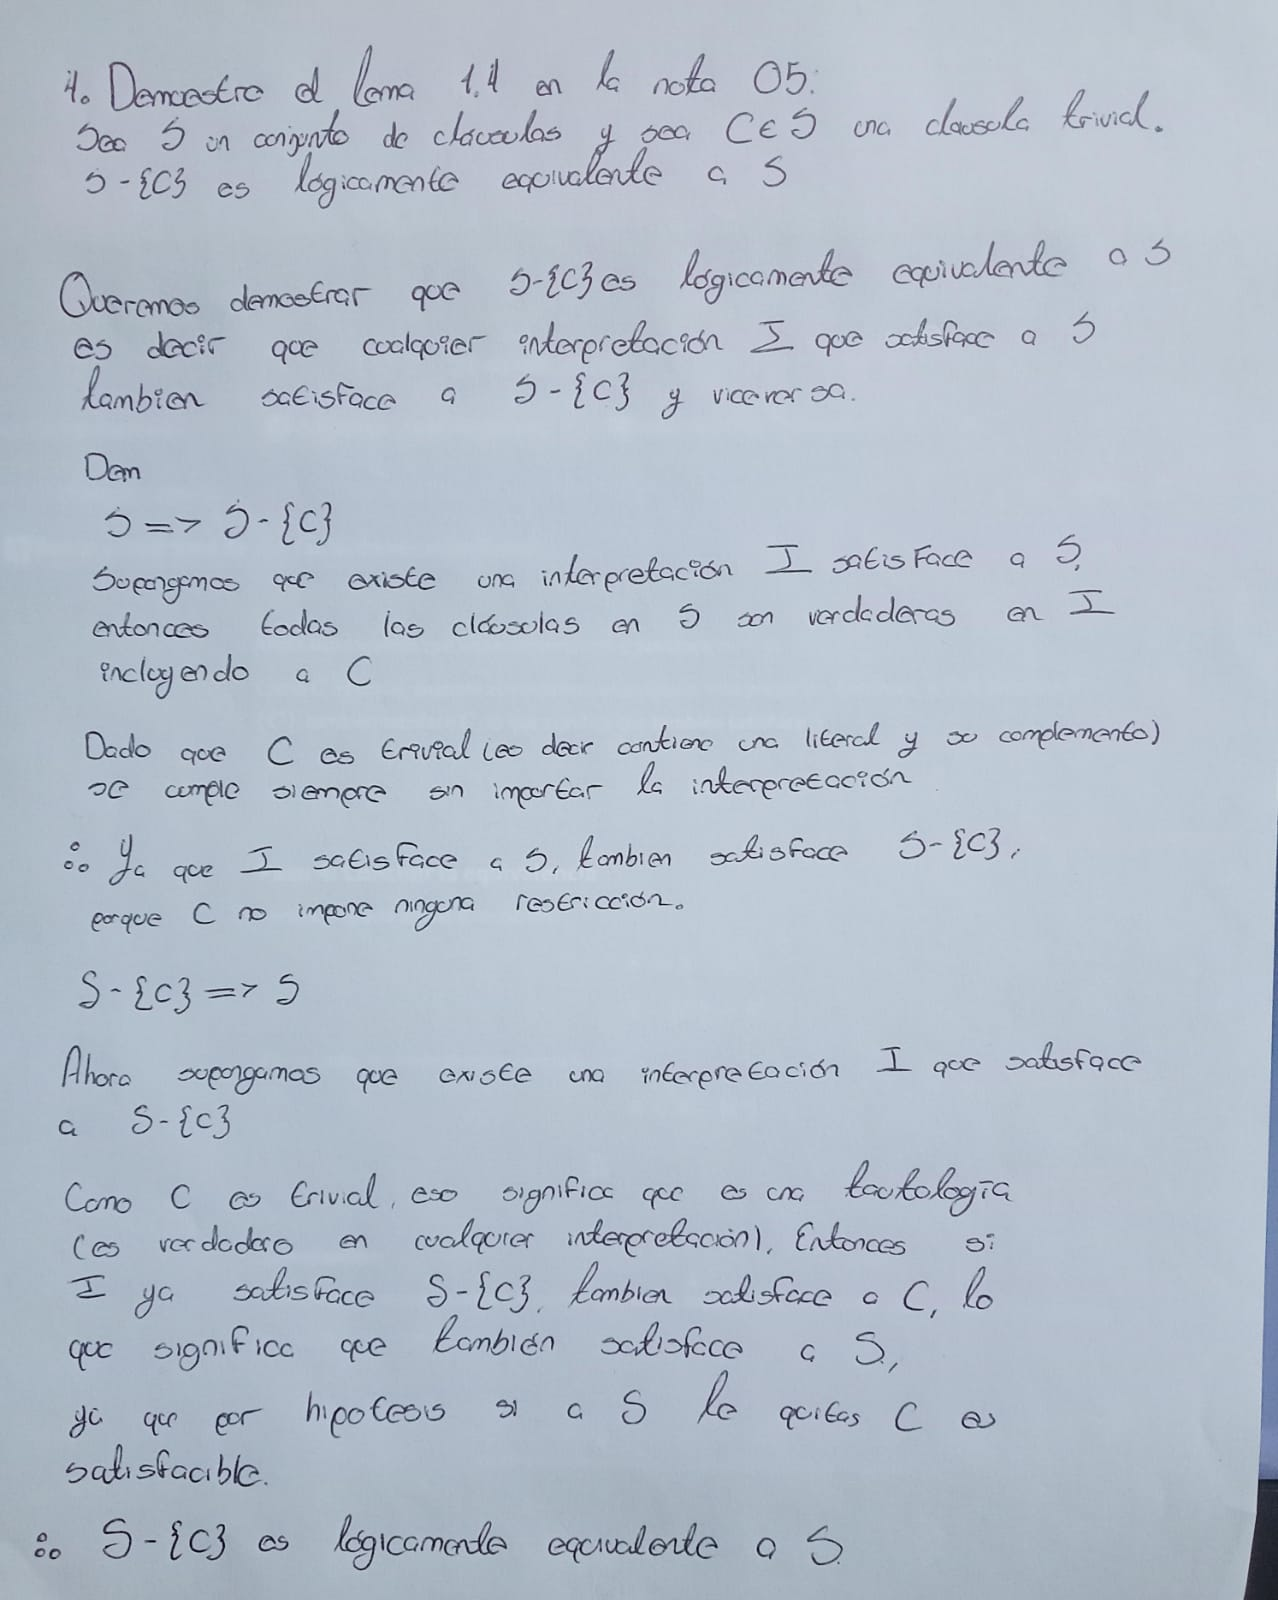
\includegraphics[width=\textwidth,height=0.8\textheight,keepaspectratio]{ejercicio4.png}
    \end{center}
    
    \newpage
    
  % ---- Ejercicio 5 ----
  \item (1.5 pts.) Demuestre que una disyunción de literales $\ell_1 \lor \dots \lor \ell_m$ es válida si y sólo si existen $1 \leq i, j \leq m$ tal que $\ell_i$ es $\neg \ell_j$.

    \begin{center}
      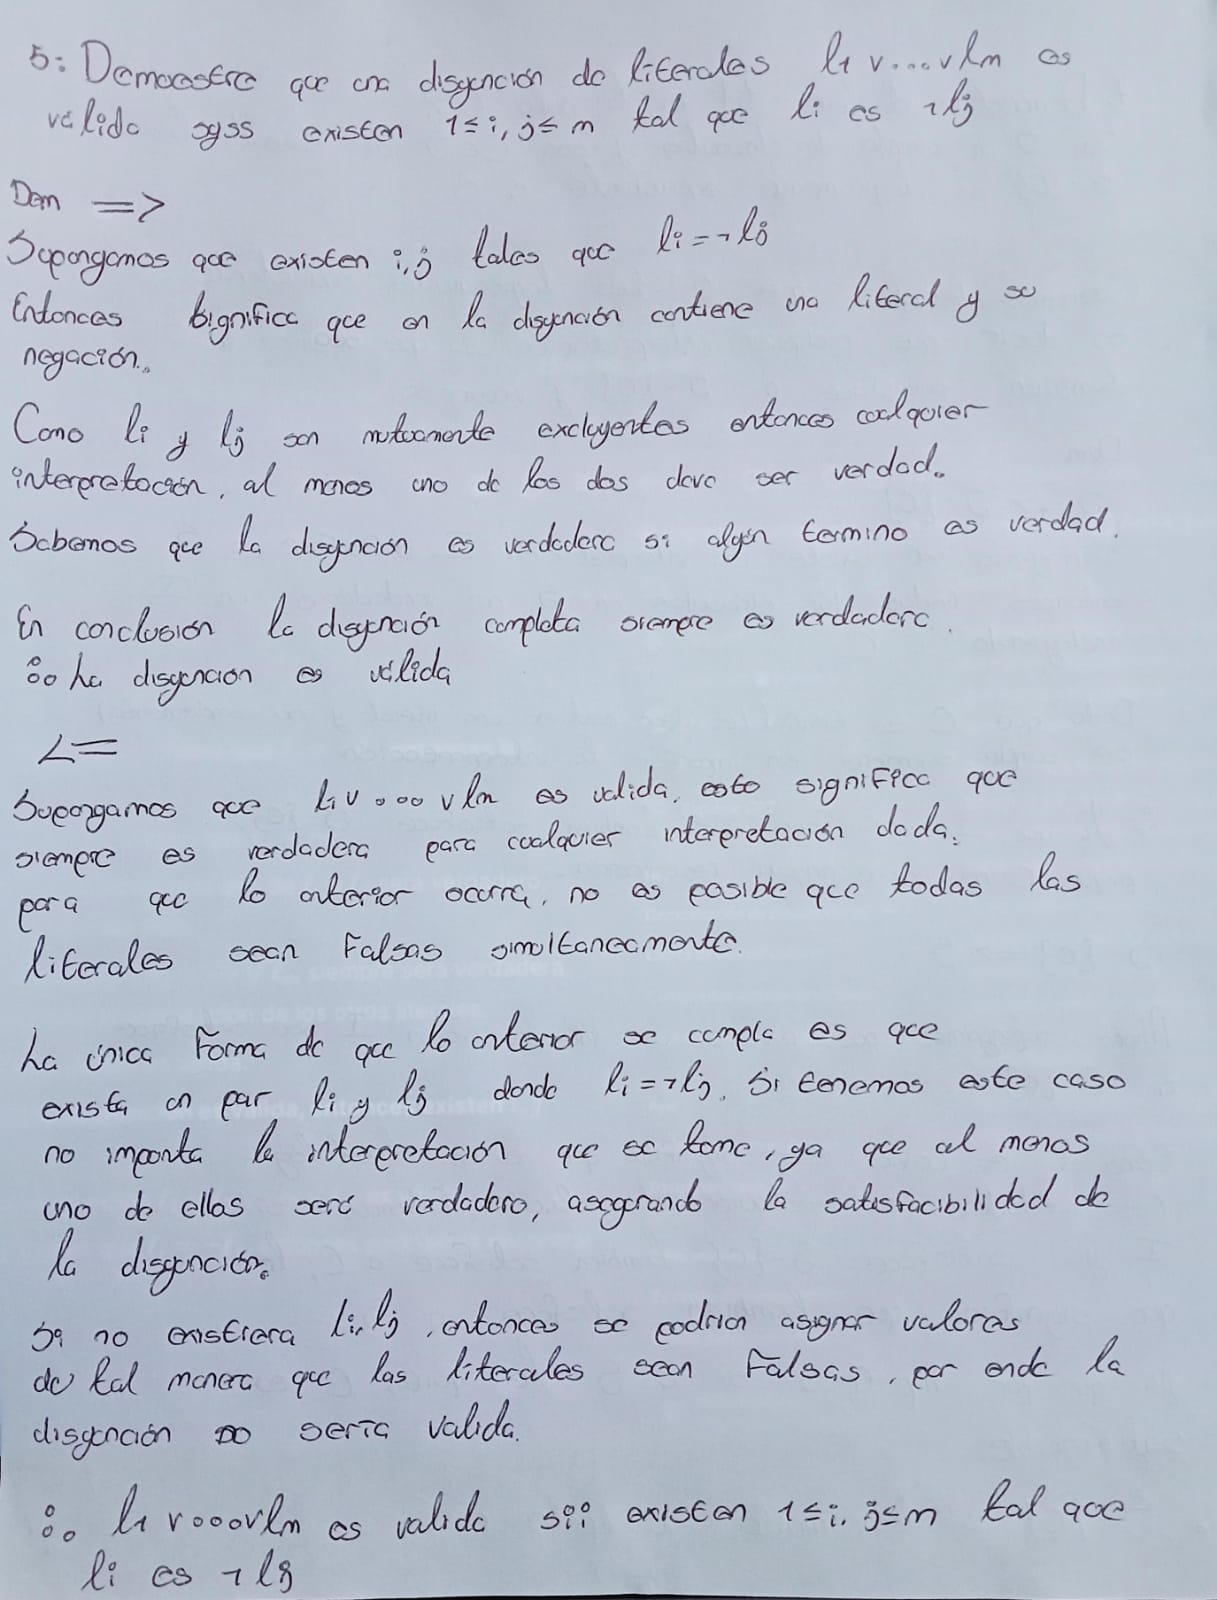
\includegraphics[width=\textwidth,height=0.8\textheight,keepaspectratio]{ejercicio5.png}
    \end{center}

    \newpage

  % ---- Ejercicio 6 ----
  \item (1 pts.) Realice las siguientes sustituciones:
  
  \begin{enumerate}[label=\alph*)]
  \item $\Big(\forall x .\big( Q(w,y,x) \wedge P(f(x),w,b) \big) \Big)[y,w:=f(w),g(x)]$\\
    \\
    Distribuimos $[y,w:=f(w),g(x)]$ a cada predicado
    \[
    \hspace{-1cm}
    \forall x .\big( Q(w, y, x)[y,w:=f(w),g(x)] \; \wedge \; P(f(x), w, b)[y,w:=f(w),g(x)] \big)
    \]
    Aplicamos la sustituci\'{o}n \'{u}nicamente en las variables no ligadas como $w$ y $y$
    \[
    \hspace{-0.5cm}
    = \forall x .\big( Q(g(x), f(w), x) \; \wedge \; P(f(x), g(x),b) \big)
    \]
    Por lo que el resultado final simplemente es
    \[
    \hspace{-0.5cm}
    \forall x .\big( Q(g(x), f(w), x) \; \wedge \; P(f(x), g(x),b) \big)
    \]
    
  \item $\Big(\begingroup\colorlet{savedleftcolor}{.}\color{red}\big(\color{savedleftcolor}\forall v .\forall w . \big( P (u, v, x) \wedge R(a, x) \wedge Q(u, w) \big)\color{red}\big)\endgroup [x, u := v, g(a, w)]\Big)[v:=f(y)]$\\
    \\
    Distribuimos $[x, u := v, g(a, w)]$ a cada predicado
    \[
    \hspace{-3cm}
    = \Big(\forall v .\forall w . \big( P (u, v, x) [x, u := v, g(a, w)]\;
    \wedge \; R(a, x) [x, u := v, g(a, w)]\;
    \wedge \; Q(u, w) [x, u := v, g(a, w)] \big)\Big)[v:=f(y)]
    \]
    Aplicamos la sustituci\'{o}n \'{u}nicamente en las variables no ligadas como $u$ y $x$
    \[
    \hspace{-1.5cm}
    = \Big(\forall v .\forall w .
    \big( P (g(a, w), v, v)\;
    \wedge \; R(a, v)\;
    \wedge \; Q(g(a, w), w) \big)\Big)[v:=f(y)]
    \]
    Ahora, n\'{o}tese que no es posible aplicar $[v:= f(y)]$ pues v es una variable que est\'{a} ligada, por lo que el resultado final es
    \[
    \hspace{-0.5cm}
    \forall v .\forall w . \big( P (g(a, w), v, v)\; \wedge \; R(a, v)\; \wedge \; Q(g(a, w), w) \big)
    \]
  \end{enumerate}

  \bigskip
  
  % ---- Ejercicio 7 ----
  \item (1 pts.) ¿Cuál es la mejor traducción para: {\em Se siente bien feo cuando se muere algo adorable que querías mucho}? Donde: $S(x)$: $x$ se siente bien feo;  $M(x)$: $x$ se muere; $A(x)$: $x$ es adorable y $Q(x,y)$: $x$ quiere mucho a $y$.
	\begin{enumerate}[label=\alph*)]
	\item $\forall x\Big(S(x)\vee \forall y\ \neg\big(M(y)\wedge Q(y,x)\wedge A(y)\big)\Big)$
	\item $\forall x\Big(\forall y \big(\neg M(y)\imp (Q(y,x)\imp \neg A(y))\big)\vee S(x)\Big)$
	\item $\forall x\Big(\neg S(x) \imp \forall y \big(M(y)\wedge Q(x,y)\imp\neg A(y)\big)\Big)$
	\item $\forall x\Big(\forall y\big(A(y)\wedge( Q(x,y) \wedge M(x)\big)\imp S(x)\Big)$
	\end{enumerate}

        \bigskip
        % -- Respuesta --
        La respuesta correcta es la $d)\; \forall x\Big(\forall y\big(A(y)\wedge( Q(x,y) \wedge M(x)\big)\imp S(x)\Big)$. Por simple descarte del resto de incisos, pues $a)$ no es posible pues niega que $M(y)$, $Q(y, x)$ y $A(y)$, nuestros predicados se cumplan, los predicados que afirman nuestro enunciado, es decir $\neg (M(y) \land Q(y, x) \land A(y) := No sucede que 'y' se muere ni 'y' quiere a 'x' ni que 'y' sea adorable$.\\
        Del mismo modo con $b)$ que niega directamente $A(y)$, pues tenemos $\neg A(y) := y NO es adorable$, y c) que igual niega uno de nuestros predicados definidos, $\neg S(x) := x NO se siente bien feo$.
        Por eso $a), b)$ y $c)$ no hacen una fiel traducci\'{o}n al enunciado propuesto.
    
    % ---- Ejercicio 8 ----
    \item (1 pt.) En una isla habitada por ingleses, funcionan tres clubes. ¿Cuál simbolización expresa mejor la siguiente afirmación? {\it Cualesquiera dos clubes tienen un socio en común.} Donde: $C(x)$: $x$ es un club; $S(x,y)$: $x$ es socio de $y$.
      \begin{enumerate}[label=\alph*)]
         \item $\exists x\  \exists y\ \exists z\ \big(x\neq y \wedge C(x) \wedge C(y) \wedge S(z,x) \wedge S(z,y)\big)$
	 \item $\exists z\ \forall x\  \forall y\ \big((x\neq y \wedge C(x) \wedge C(y)) \imp (S(z,x) \wedge S(z,y))\big)$
	 \item $\forall x\  \forall y\ \big((x\neq y \wedge C(x) \wedge C(y)) \imp \exists z\ (S(z,x) \vee S(z,y))\big)$
	 \item $\forall x\  \forall y\ \exists z\ \big((x\neq y \wedge C(x) \wedge C(y)) \imp (S(z,x) \wedge S(z,y))\big)$
      \end{enumerate}
      
      Para los dos últimos incisos tome en cuenta estas equivalencias:
      \[\arraycolsep=1.4pt\def\arraystretch{1.5}
      \begin{array}{lcl}
        \vp \imp \psi &\equiv& \neg\vp \vee\psi\\
        \vp \imp \psi &\equiv& \neg\psi \imp \neg\vp\\
        \neg(\vp\wedge\psi) &\equiv& \neg\vp\vee\neg\psi\\
        \neg(\vp\vee\psi) &\equiv& \neg\vp\wedge\neg\psi\\
        \neg\forall x\;\vp &\equiv& \exists x\;\neg\vp\\
        \neg\exists x\;\vp &\equiv& \forall x\;\neg\vp
      \end{array}
      \]

      \bigskip
      % -- Respuesta
      La respuesta correcta es la $d)\; \forall x\  \forall y\ \exists z\ \big((x\neq y \wedge C(x) \wedge C(y)) \imp (S(z,x) \wedge S(z,y))\big)$.
      La afirmación nos dice {\it Cualesquiera dos clubes tienen un socio en común}, esto lo podemos interpretar de la forma: {\it para cualquier par de los 3 clubes que puedas tomar existe al menos una persona que es socio de ambos}.\\
      En este caso la opción que representa la oración es el inciso $d)$ ya que en el inciso $a)$ se afirma que existe al menos un par de clubes con un solo socio en común sin tomar en cuenta todos los pares posibles.\\
      En el inciso $b)$ se afirma que, {\it para todos los pares posibles de clubes hay un socio común}.
      En el inciso $c)$ nos dice que {\it para cualquier par de clubes distintos existe un socio de al menos uno de ellos}.\\
      Y el inciso $d)$ afirma que {\it para cualquier par de clubes distintos, existe un socio de ambos}, lo que coincide con el enunciado original.
      
\end{enumerate}
\end{document}
